\documentclass[usenames,dvipsnames,notes,11pt,aspectratio=169,hyperref={colorlinks=true, linkcolor=blue}]{beamer}
\usepackage{ifthen}
\usepackage{xcolor}
\usepackage{pgfplots}
\usepackage{amsmath}
\usepackage{centernot}
\usepackage{pifont}
\usepackage{tabularx}
\usepackage{makecell}
\usepackage{cuted}
\usepackage{booktabs}
\usepackage{array}
\usepackage{textcomp}
\usepackage{setspace}
\usepackage{xspace}
\usepackage{subcaption}
\usepackage{tikz}
\usepackage{pdfcomment}
%\newcommand{\pdfnote}[1]{\marginnote{\pdfcomment[icon=note]{#1}}}
\newcommand{\pdfnote}[1]{}

\usepackage{pgfpages}
%\setbeameroption{show notes on second screen}


\input ../beamer-style
\input ../std-macros
\input ../macros

\newcommand{\pt}{\partial}

\AtBeginSection[]
{
    \begin{frame}
        \frametitle{Table of Contents}
        \tableofcontents[currentsection]
    \end{frame}
}
\parskip=10pt

\title[CSCI-GA.2590]{Language models}
\author[He He]{He He
}
\institute[NYU]{
    
\includegraphics[height=1cm]{../figures/nyu-logo}\\
}
\date{April 4, 2023}

\begin{document}
\begin{frame}
\titlepage
\end{frame}

\begin{frame}
    {What do language models do?}

    \begin{columns}
        \begin{column}{0.5\textwidth}
            \begin{itemize}
                \item Answer questions 
                \item Summarize documents 
                \item Write programs 
                \item Prove theorems
                \item ...
            \end{itemize}
        \end{column}
        \begin{column}{0.5\textwidth}
            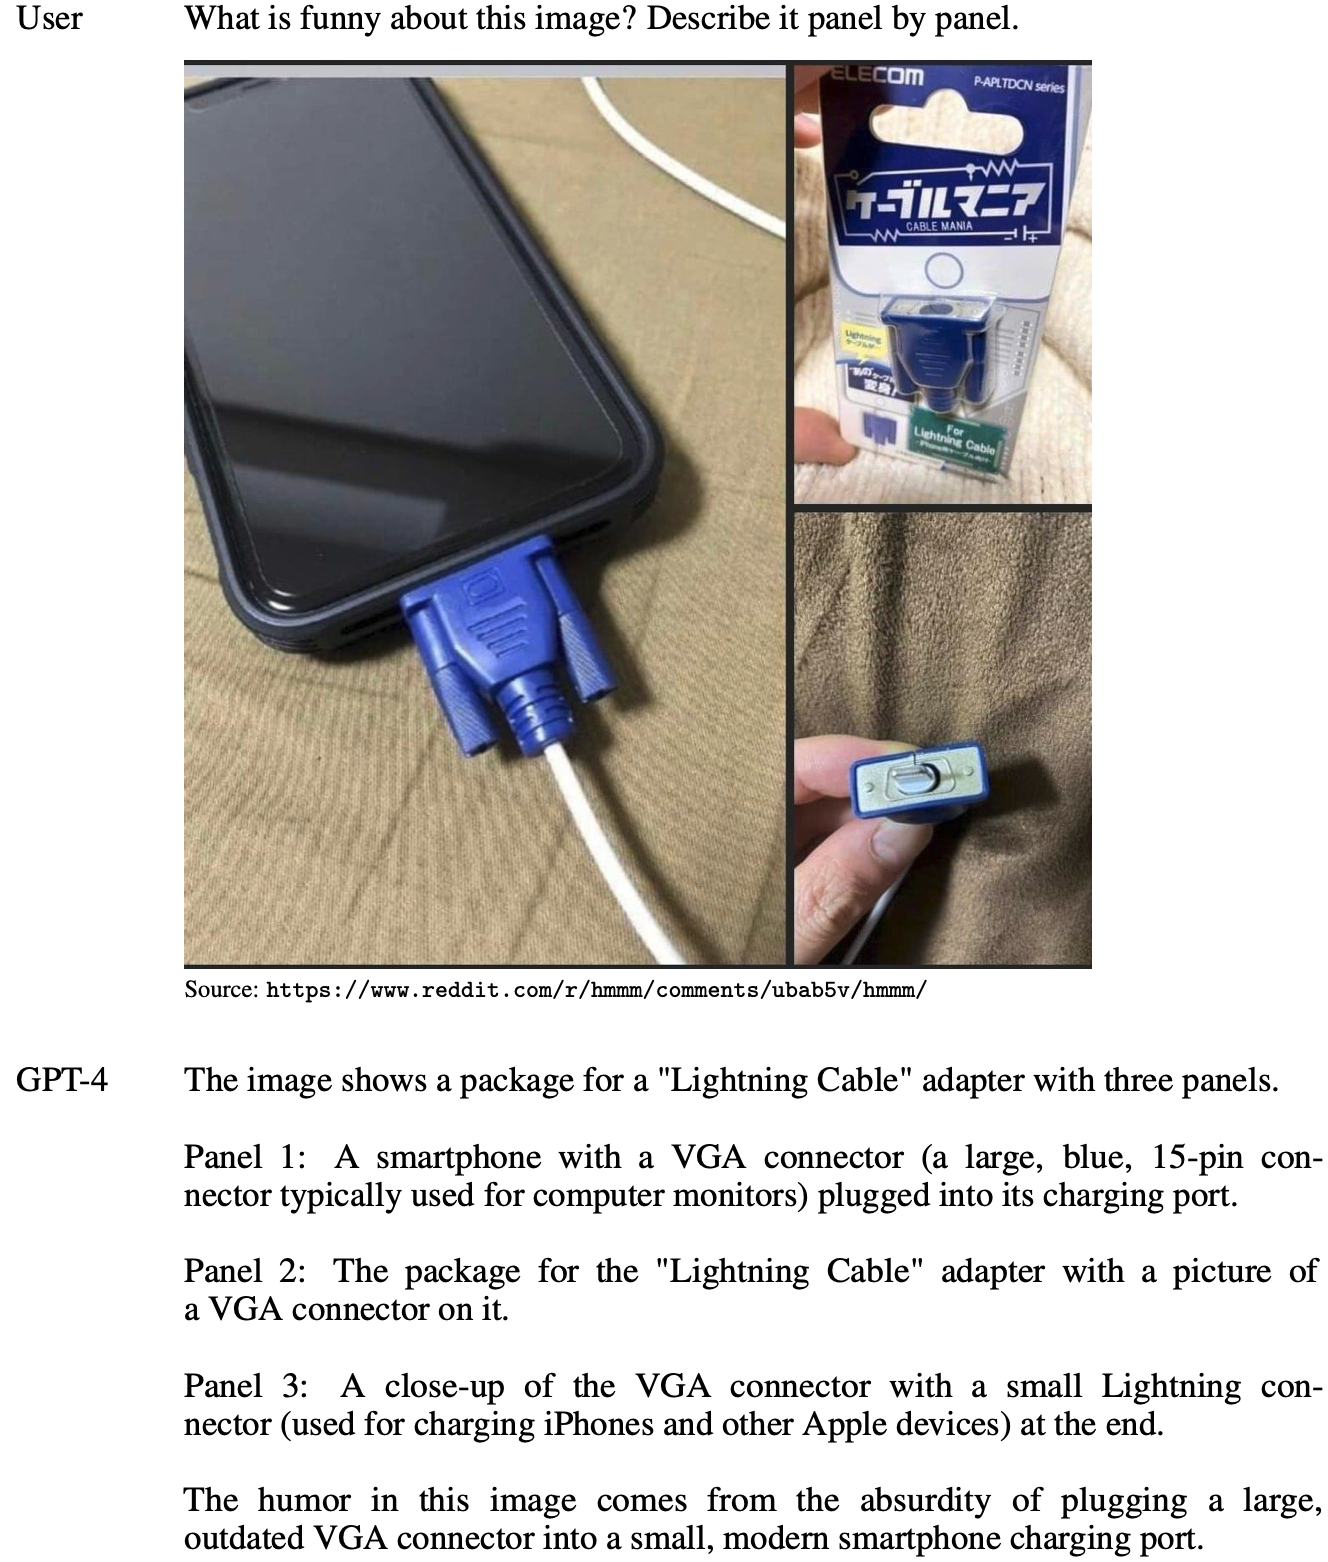
\includegraphics[width=\textwidth]{figures/gpt4}
        \end{column}
    \end{columns}
\end{frame}

\begin{frame}
    {Dial back ten years}
    Which output is more likely?
    \begin{itemize}
        \item Speech recognition
            \begin{itemize}
                \item[] the \textit{tail} of a dog
                \item[] the \textit{tale} of a dog
            \end{itemize}
            \begin{itemize}
                \item[] It's not easy to \textit{wreck a nice beach}. 
                \item[] It's not easy to \textit{recognize speech}. 
                \item[] It's not easy to \textit{wreck an ice beach}.
            \end{itemize}
        \item Machine translation 
            \begin{itemize}
                \item[] He sat on the \textit{table}.
                \item[] He sat on the \textit{figure}.
            \end{itemize}
            \begin{itemize}
                \item[] Such a Europe would \textit{the rejection of any} ethnic nationalism. 
                \item[] Such a Europe would \textit{mark the refusal of all} ethnic nationalism. 
            \end{itemize}
    \end{itemize}
    \pdfnote{
        In earlier systems of speech recognition and machine translation,
        the acousitic model and the translation model would produce multiple rough translations, and the language model is used to reweight these outputs by how likely they are English sentences.
    }
\end{frame}

\begin{frame}
    {Outline}
    Plan for today:

    From n-gram language models to GPT
\end{frame}

\begin{frame}
    {Problem formulation}
    \textbf{Goal}: Assign probabilities to a sequence of tokens, e.g., \\
    \begin{itemize}[<+->]
        \item $p(\text{the red fox jumped})
            \onslide<+->{\gg} p(\text{the green fox jumped})$
        \item $p(\text{colorless green ideas sleep furiously})
            \onslide<+->{\gg} p(\text{furiously sleep ideas green colorless})$
    \end{itemize}

    \onslide<.->{
        Formulation:\\}
    \begin{itemize}[<+->]
        \item \textbf{Vocabulary}: a set of symbols $\sV$, e.g.\\
            \indent $\pc{\text{fox}, \text{green}, \text{red}, \text{jumped}, \text{a}, \text{the}}$
        \item \textbf{Sentence}: a {finite} sequence over the vocabulary $x_1 x_2 \ldots x_n \in \sV^n$ where $n\ge 0$ %(empty sequence when $n=0$)
        \item The set of all sentences (of varying lengths): $\sV^*$ 
        \item Assign a probability $p(x)$ to all sentences $x\in\sV^*$. 
    \end{itemize}
    \pdfnote{
        red > green: green fox is very rare.
        Grammatically correct sentences is more likely than gibberish.
    }
    \pdfnote{
        Language models tell us how likely we'll encounter a sentence in English. 
        A common misconception is that low probability under an LM means ungrammatical text. However, a sentence can be rare due to many reasons, it could contain rare words, being ungrammatical, or doesn't make any sense. Low probability doesn't necessarily mean ungrammaticality.
    }
    \pdfnote{
        Today, our task is to model this distribution and estimate its params given a corpus.
    }
\end{frame}

\begin{frame}
    {A naive solution}
    \begin{itemize}[<+->]
        \itemsep1em
        \item \textbf{Training data}: a set of $N$ sentences %: $D=\pc{x^{(i)}}_{i=1}^N$
            %\begin{itemize}[<.->]
            %    \item Notation: $x^{\textstyle\text{(instance id)}}_{\textstyle\text{token id}}$
            %\end{itemize}
        \item \textbf{Modeling}: use a multinomial distribution as our language model 
            $$
            p_s(x) = \frac{\text{count}(x)}{N} \;.
            $$
            (Exercise: Check that $\sum_{x\in\sV^*}p_s(x) = 1$.)
        \item Is $p_s$ a good LM?\pause
            \begin{itemize}
                \item Most sentences only occur once. \hspace{2cm}\red{\textit{sparsity issue}}
                \item Need to restrict the model. 
            \end{itemize}
    \end{itemize}
    \pdfnote{
        Let's consider a multinomial distribution over the sentences,
        where each sentence is an event, and we estimate the probability of each sentence by its fraction in the corpus.
        Specifically, the count of its occurence divided by the total number of sentences.
    }
    \pdfnote{
        This says that our model is too flexible. The number of parameters are the total number of sentences, which increases exponentially with the vocab size. It can approximate any distribution but we won't be able to estimate the model with limited data.
    }
\end{frame}

\begin{frame}
    {Simplification 1: sentence to tokens}
    Solve a smaller problem: model probability of each token

    Decompose the joint probability using the \textbf{probability chain rule}:
            \begin{align*}
                \onslide<+->{
            p(x) &= p(x_1, \ldots, x_n) \\
                &= p(x_1)p(x_2\mid x_1)p(x_3\mid x_1, x_2)\ldots p(x_n\mid x_{1}, \ldots, x_{n-1}) \\
            }
                \onslide<+->{
                & (\text{Doesn't have to go from left to right}) \\
                &= p(x_n)p(x_{n-1}\mid x_n) \ldots p(x_1\mid x_{2},\ldots, x_n)
            }
            \end{align*}
            \vspace{-1em}

    \begin{itemize}[<+->]
        \item Problem reduced to modeling conditional token probabilities\\
            the red fox $\rightarrow$ jumped
        \item The left-to-right decomposition is also called an \textbf{autoregressive model}
        %\item Number of outcomes: $|\sV^*|$ (sentences) to $|\sV|$ (symbols)
        \item This is a classification problem we have seen
        \item But there is still a large number of contexts!
    \end{itemize}

\end{frame}

\begin{frame}
    {Simplification 2: limited context}
    Reduce dependence on context by the \textbf{Markov assumption}:\\
    \begin{itemize}
        \item First-order Markov model
            \begin{align*}
                p(x_i\mid x_1,\ldots, x_{i-1}) &= p(x_i\mid x_{i-1}) \\
                p(x) &= \prod_{i=1}^n p(x_i\mid x_{i-1})
            \end{align*}
        \item Number of contexts? \pause $|\sV|$
        \item Number of parameters? \pause $|\sV|^2$
    \end{itemize}
\end{frame}

\begin{frame}
    {Model sequences of variable lengths}

    %Beginning of a sequence:\\
    %$$
    %p(x_1\mid x_{1-1}) = ?
    %$$
    Assume each sequence starts with a special \textbf{start symbol}: $x_0=*$.
    \medskip

    Assume that all sequences end with a \textbf{stop symbol} \texttt{STOP}, e.g.
    \begin{align*}
        &\quad p(\text{the}, \text{fox}, \text{jumped}, \texttt{STOP})\\
         &= p(\text{the}\mid {\color{blue}*})
         p(\text{fox}\mid \text{the})
         p(\text{jumped}\mid \text{fox})
         p({\color{blue}\texttt{STOP}}\mid \text{jumped})
    \end{align*}

    \pause
    {What if we don't have the stop symbol?}\\
    \begin{itemize}
        \item Which one is larger: $p(\text{the fox})$ or $p(\text{the fox jumped})$?
    \end{itemize}

    %\pause
    %LM with the \texttt{STOP} symbol:\\
    %\begin{itemize}
    %    \item Vocabulary: $\texttt{STOP} \in \sV$
    %    \item Sentence: $x_1 x_2 \ldots x_n \in \sV^n$ for $n\ge 1$ and $x_n=\texttt{STOP}$.
    %\end{itemize}
    %\pdfnote{
    %    Accordingly, we'll revise our problem formulation to include the stop symbols.
    %}
\end{frame}

\begin{frame}
    {N-gram LM}
    \begin{itemize}
        \item Unigram language model (no context):
            $$
            p(x_1,\ldots, x_n) = \prod_{i=1}^n p(x_i) \;.
            $$
        \item Bigram language model ($x_0=*$):
            $$
            p(x_1,\ldots, x_n) = \prod_{i=1}^n p(x_i\mid x_{i-1}) \;.
            $$
        %\item Trigram language model ($x_{-1}=*,x_0=*$):
        %    $$
        %    p(x_1,\ldots, x_n) = \prod_{i=1}^n p(x_i\mid x_{i-2}, x_{i-1}) \;.
        %    $$
        \item $n$-gram language model:
            $$
            p(x_1,\ldots, x_m) = \prod_{i=1}^m p(x_i\mid \underbrace{
                x_{i-n+1},\ldots, x_{i-1}
            }_{\textstyle\text{previous $n-1$ words}} )
            \;.
            $$
    \end{itemize}
\end{frame}

%\begin{frame}
%    {Practical issues}
%    \begin{itemize}
%        \itemsep1em
%        \item Use $n-1$ start symbols for $n$-gram models
%        \item Trigram features are often used in classification
%        \item Higher-order models (4/5-grams) are used for MT when large corpus is available
%        \item All computation is done in the log space to avoid underflow
%    \end{itemize}
%\end{frame}

%\begin{frame}
%    {Parameter estimation}
%    \begin{itemize}
%        \itemsep1em
%        \item Data: a corpus $\pc{x^{(i)}}_{i=1}^N$ where $x\in\sV^n$ denote a sequence.
%        \item Model: bigram LM $p(w\mid w')$ for $w,w'\in\sV$.
%            $$
%            p(w\mid w') = \theta_{w\mid w'} \quad \text{multinomial distribution}
%            $$
%            where $\sum_{w\in\sV}p(w\mid w') = 1 \quad \forall w'\in\sV$.
%    \end{itemize}
%
%\end{frame}

\begin{frame}
    {Parameter estimation}
    Maximum likelihood estimation over a corpus (a set of sentences):\\
    \begin{itemize}
        \item Unigram LM
            $$
            {p}_{\text{MLE}}(x) = \frac{\text{count}(w)}{\sum_{w\in\sV}\text{count}(w)}
            $$
        \item Bigram LM
            $$
            {p}_{\text{MLE}}(w\mid w') =
            \frac{\text{count}(w,w')}{\sum_{w\in\sV}\text{count}(w,w')}
            $$
        \item In general, for n-gram LM,
            $$
            {p}_{\text{MLE}}(w\mid c) =
            \frac{\text{count}(w,c)}{\sum_{w\in\sV}\text{count}(w,c)}
            $$
            where $c\in \sV^{n-1}$.
    \end{itemize}
\end{frame}

\begin{frame}
    {Example}
    \begin{itemize}
        \item Training corpus (after tokenization)
            \begin{itemize}
                \item[] $\pc{\text{The fox is red},
                    \text{The red fox jumped},
                    \text{I saw a red fox}
                    }$
            \end{itemize}
        \item Collect counts
            \begin{itemize}
                \item[] $\text{count}(\text{fox})=3$
                \item[] $\text{count}(\text{red})=3$
                \item[] $\text{count}(\text{red}, \text{fox})=2$
                \item[] $\ldots$
            \end{itemize}
        \item Parameter estimates
            \begin{itemize}
                \item[] $\hat{p}(\text{red}\mid\text{fox})=\pause 2/3$
                \item[] $\hat{p}(\text{saw}\mid\text{i})=\pause 1/1$
            \end{itemize}
        \pause
    \item What is the probability of ``The fox saw I jumped''?\pause \hspace{2em} \red{Zero probability on unseen n-grams}
        \pdfnote{
            Zero probability: OOV words or unseen n-grams.
        }
    \end{itemize}
\end{frame}

\begin{frame}
    {Generating text from an n-gram model}
    \begin{enumerate}
        \item Initial condition: $\text{context}=\ast$
        \item Iterate until next\_word is \texttt{STOP}:
            \begin{enumerate}
                \item $\text{next\_word} \sim p(\cdot \mid \text{context}[:-(n-1)])$
                \item $\text{context}  \leftarrow \text{context} + \text{next\_word}$
            \end{enumerate}
    \end{enumerate}

    \pause
    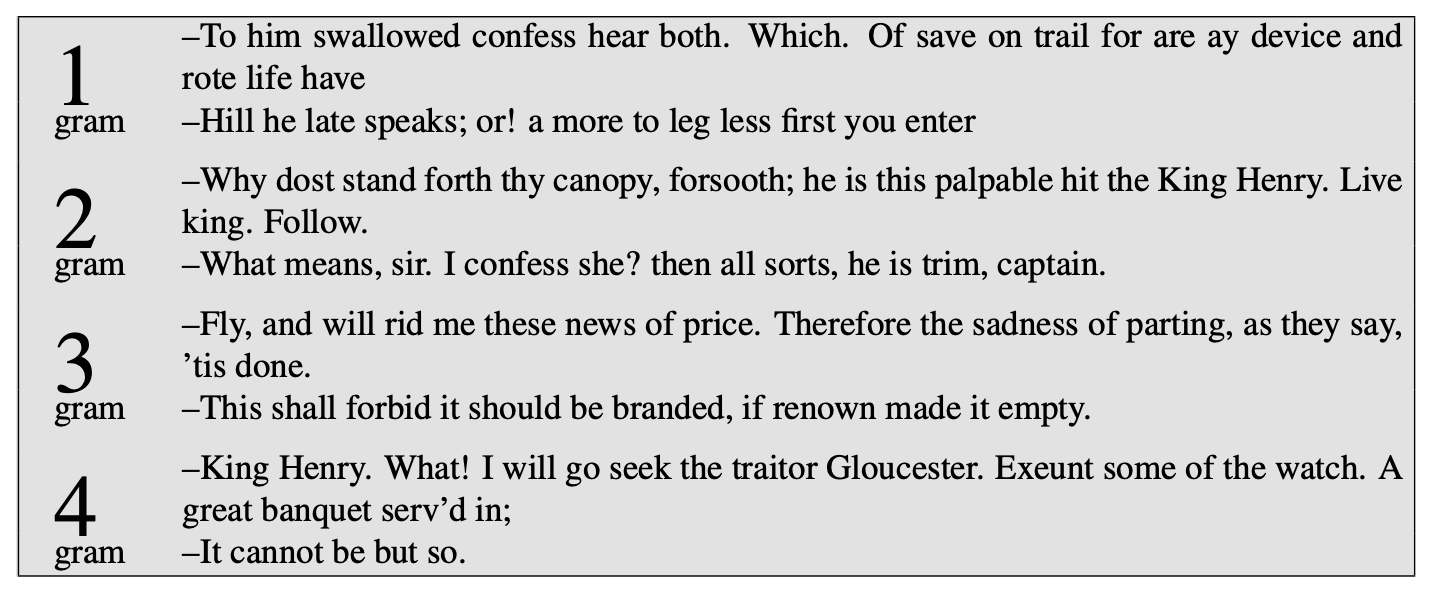
\includegraphics[height=4.5cm]{figures/ngram-sample}\\[1ex]
    What is the training data?

\end{frame}

\begin{frame}
    {Perplexity}
    What is the loss function for learning language models?
    \pause

    Held-out likelihood on test data $D$ (negative test loss):
    $$
    \ell({D}) = \sum_{i=1}^{|D|} \log p_\theta(x_i\mid x_{1:i-1}) \;,
    $$
    \vspace{-2em}
    \pdfnote{In practice, no sentence segmentation, a sequence of words, average likelihood of each word}
    \pause

    \textbf{Perplexity}:
    $$
 \text{PPL}(D) = 2^{-\frac{\ell(D)}{|D|}} \;.
 $$
    \vspace{-2em}
    \begin{itemize}
        \item Base of log and exponentiation should match
        \item Exponent is cross entropy: $H(p_{data}, p_\theta) = -\BE_{x\sim p}\log p_\theta(x)$.
            \pdfnote{Entropy is the number of bits needed to encode an event from a certain distribution.}
            \pdfnote{Cross-entropy is the number of bits needed to encode an event from a certain distribution (here p data) when your coding scheme is optimized for another distribution (here p theta).}
        \item Interpretation: a model of perplexity $k$ predicts the next word by throwing a fair $k$-sided die.
            \pdfnote{2 to the number of bits: total number of outcomes}
            \pdfnote{Sanity check: if PPL is larger than vocab size, something must be wrong.}
    \end{itemize}
\end{frame}

\begin{frame}
    {Summary}
    \textbf{Language models}: assign probabilities to sentences
    \pause

    \textbf{N-gram language models}:\\
    \begin{itemize}
        \item Assume each word only conditions on the previous $n-1$ words
        \item MLE estimate: counting n-grams in the training corpus
    \end{itemize}
    \pause

    {Evaluation} by \textbf{held-out perplexity}: how much probability mass does the model assign to unseen text 
    \pause

    Challenges:\\
    \begin{itemize}
        \item \textbf{Generalization}: sentences containing unseen n-grams have zero probability
        \item Much research in n-gram LM is dedicated to \textbf{smoothing} methods that allocate probability mass to unseen n-grams
    \end{itemize}
\end{frame}

%neural LM solves the generalization problem
%- rnn, transformer training and inference
%- improved perplexity

\begin{frame}
    {Neural language models}
    Neural networks solve the generalization problem in n-gram LMs.
    \begin{figure}
            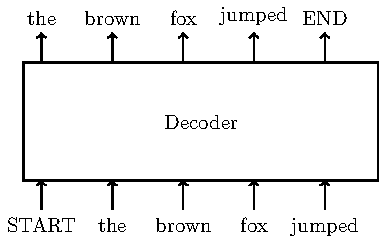
\includegraphics[height=0.5\textheight]{figures/decoder}
    \end{figure}
    \begin{itemize}
        \item A decoder-only autoregressive neural language model 
        \item Decoder can be an RNN or a transformer (with causal masking)
        \item What's the context size?
    \end{itemize}
\end{frame}

\begin{frame}
    {Early efforts on scaling neural language models}
    \begin{figure}
            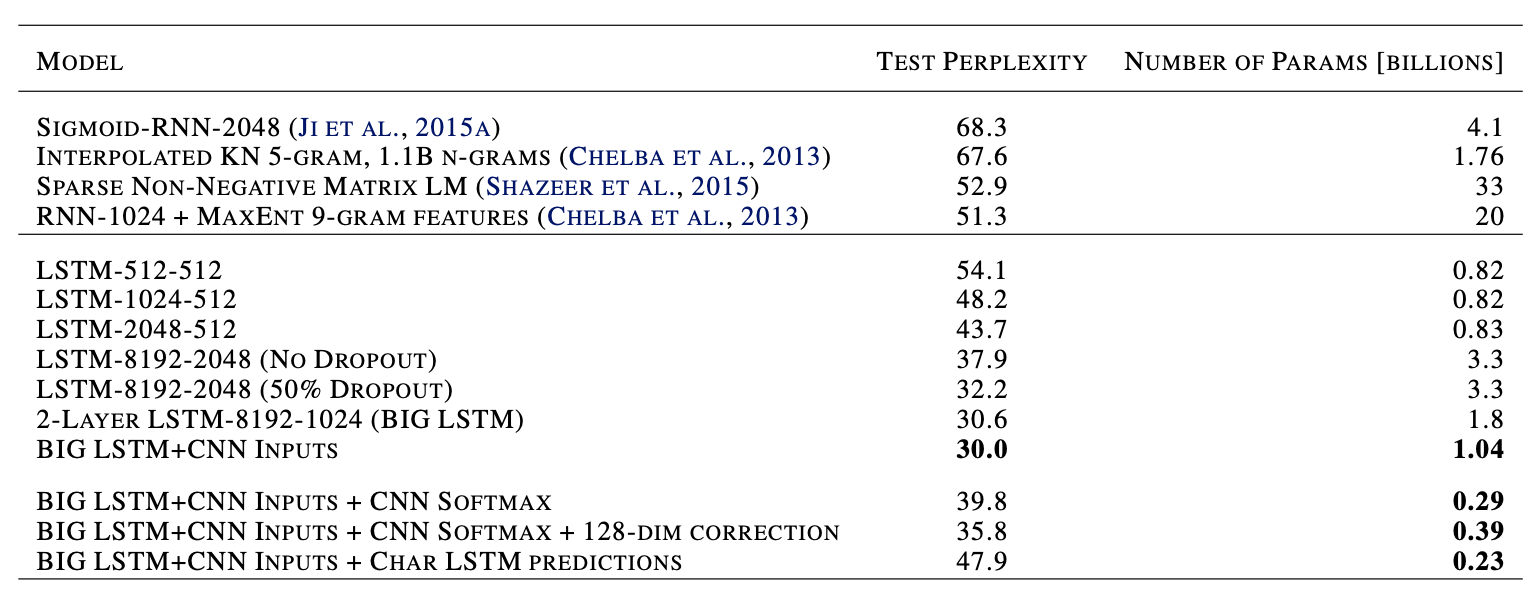
\includegraphics[width=\textwidth]{figures/lm-result}
            \caption{From \href{https://arxiv.org/pdf/1602.02410.pdf}{Exploring the Limits of Language Modeling}}
    \end{figure}
    \vspace{-1em}
    Significant improvement in held-out perplexity given similar model sizes ($\sim$1B)
\end{frame}

\begin{frame}
    {Improvement from neural language models}
    \begin{figure}
            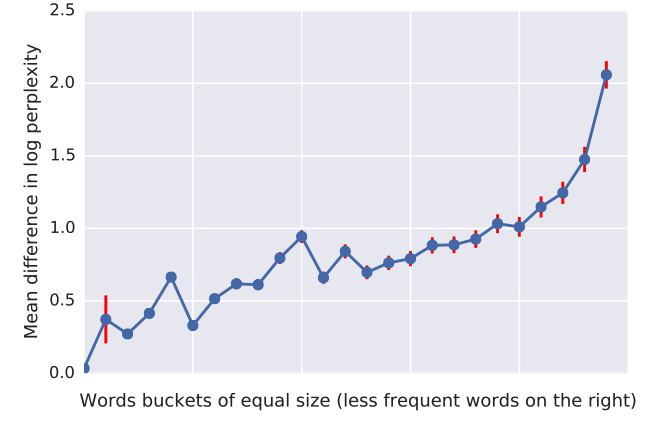
\includegraphics[width=0.45\textwidth]{figures/lm-result-2}
            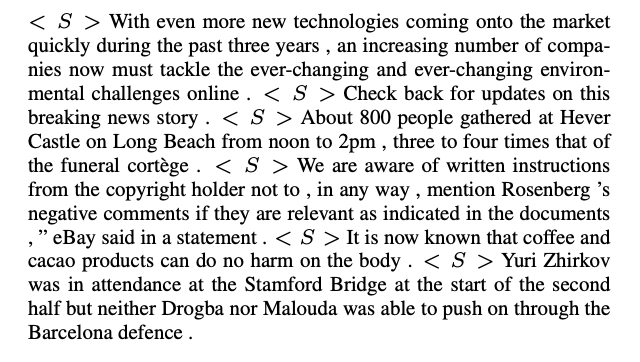
\includegraphics[width=0.5\textwidth]{figures/lm-result-3}
            \caption{From \href{https://arxiv.org/pdf/1602.02410.pdf}{Exploring the Limits of Language Modeling}}
    \end{figure}
    \vspace{-1em}
    LSTM vs KN5: improved perplexity on tail words
\end{frame}

%lm for pretraining
%- gpt vs bert
\begin{frame}
    {Recap: language modeling as pretraining}
    What can we do with a very large language model?
    \begin{itemize}
        \itemsep1em
        \item The cats that are raised by my sister \rule{1.5cm}{0.5mm} sleeping. \hfill \textit{syntax}
        \item Jane is happy that John invited \rule{1.5cm}{0.5mm} friends to his birthday party. \hfill \textit{coreference}
        \item \rule{1.5cm}{0.5mm} is the capital of Tanzania. \hfill \textit{knowledge}
        \item The boy is \rule{1.5cm}{0.5mm} because he lost his keys.  \hfill \textit{commonsense}
        \item John took 100 bucks to Vegas. He won 50 and then lost 100. Now he only has \rule{1.5cm}{0.5mm} to go home. \hfill \textit{numerical reasoning}
    \end{itemize}
    Predicting the next word entails many natural language understanding tasks
\end{frame}

\begin{frame}
    {Generative Pre-Training (GPT)}
        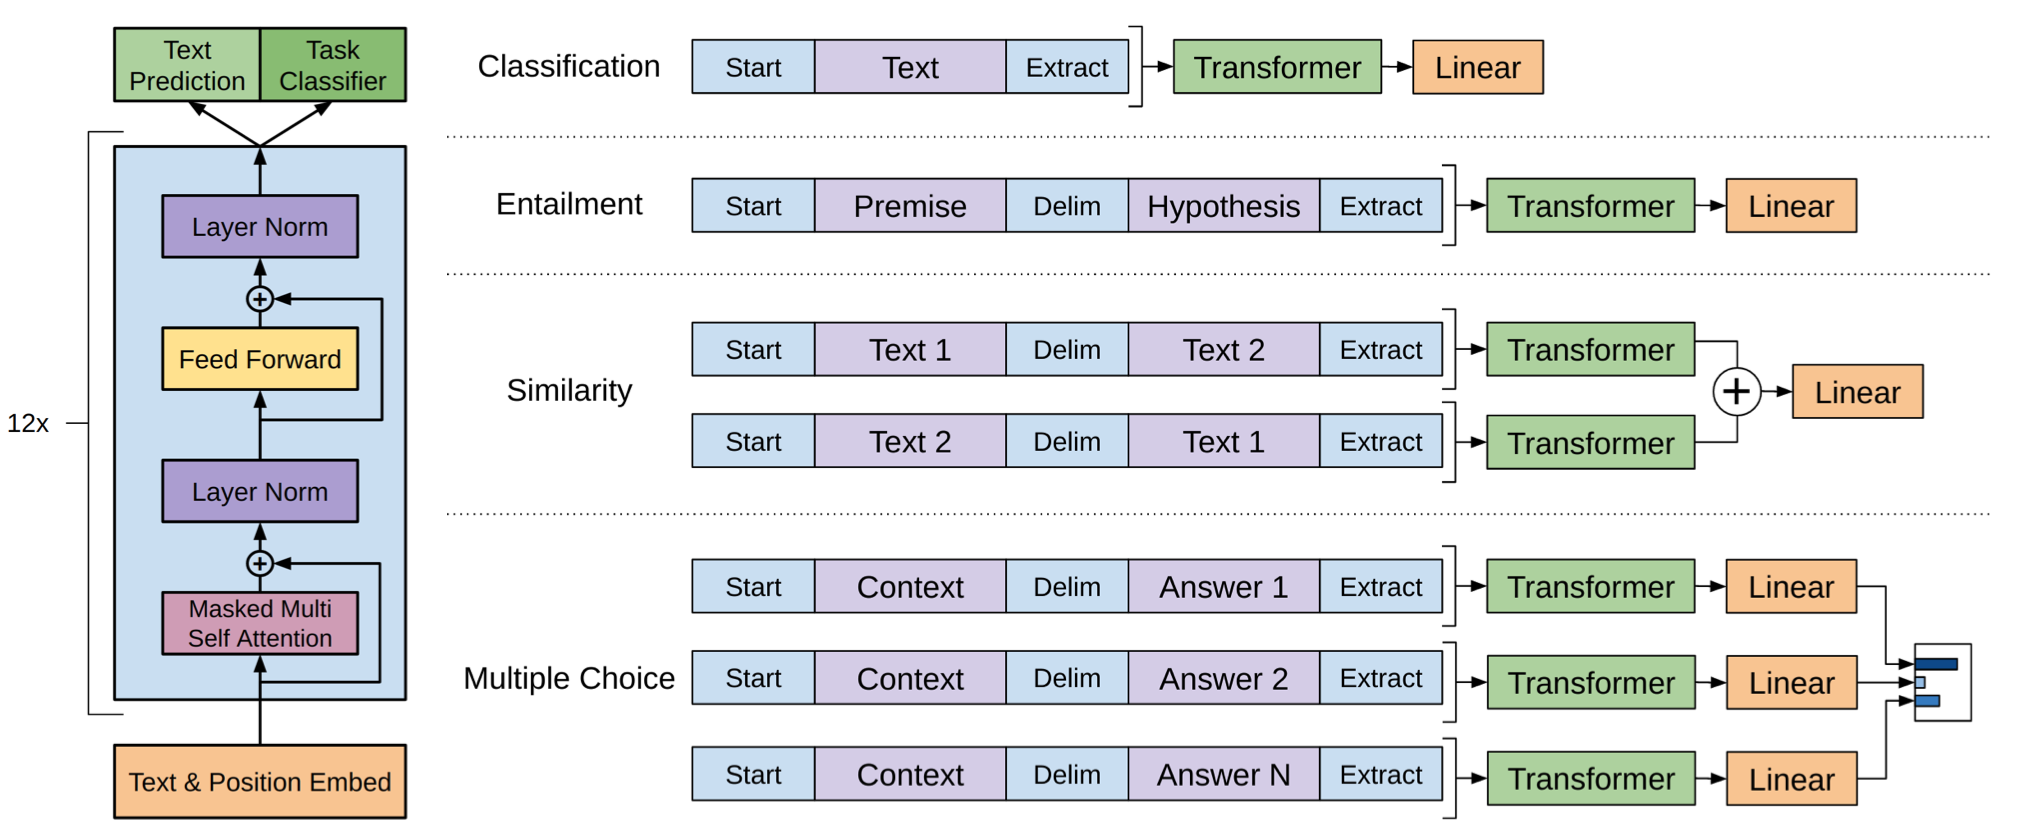
\includegraphics[width=0.9\textwidth]{figures/gpt1}

    \begin{itemize}
        \item Pretrained on Bookcorpus; 12 layer decoder-only transformer; learned position embedding; GELU activation
        \item \blue{Auxiliary LM objective} during finetuning: $L_{\text{task}} + \lambda L_{\text{LM}}$
    \end{itemize}
\end{frame}

\begin{frame}
    {Ablation studies}
    Architecture, pretraining, finetuning: which is critical?
    \begin{figure}
        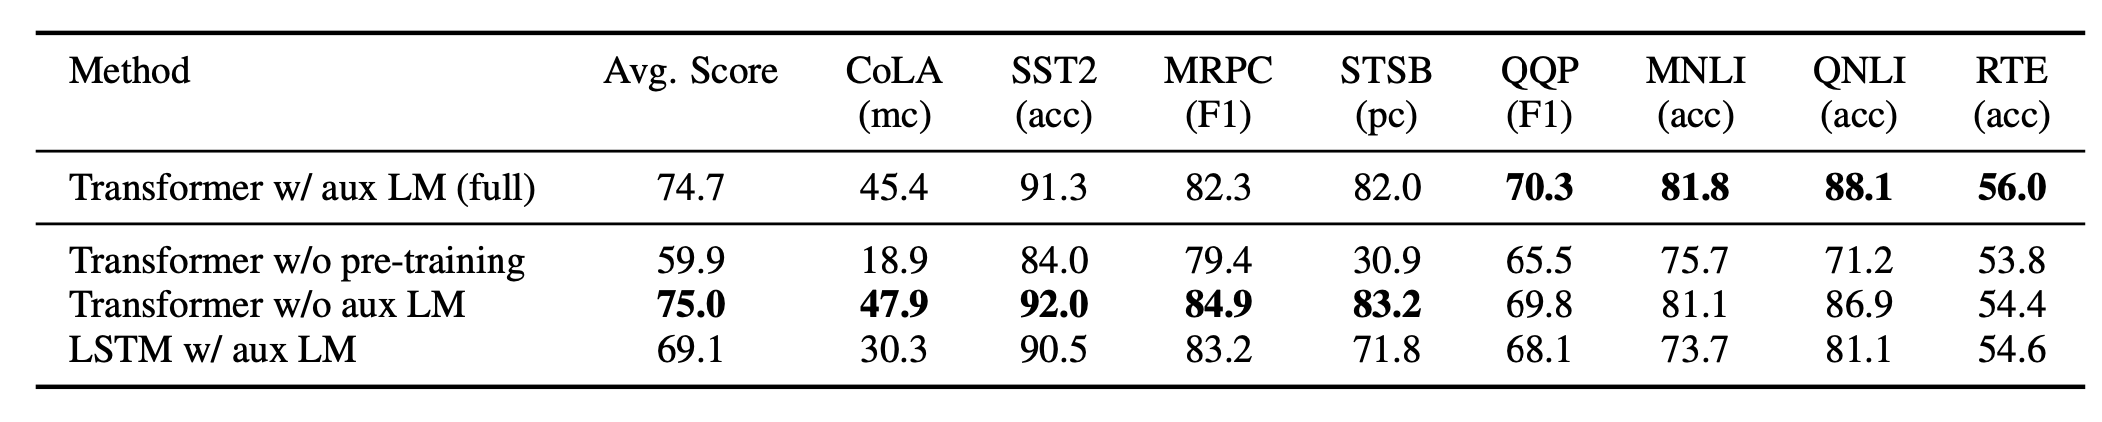
\includegraphics[width=\textwidth]{figures/gpt-ablation}
    \end{figure}
    \begin{itemize}
        \item Auxiliary objective only helps on larger datasets (MNLI, QQP)
        \item Pretrained transformer $>$ pretrained LSTM (single layer) $>$ non-pretrained transformer
    \end{itemize}
\end{frame}

\begin{frame}
    {Zero-shot behaviors}
    \textbf{Key insight}: if the model has learned to understand language through predicting next words, it should be able to perform these tasks {\em without finetuning}

    \vspace{1em}
    \pause
    \begin{columns}
        \begin{column}{0.4\textwidth}
        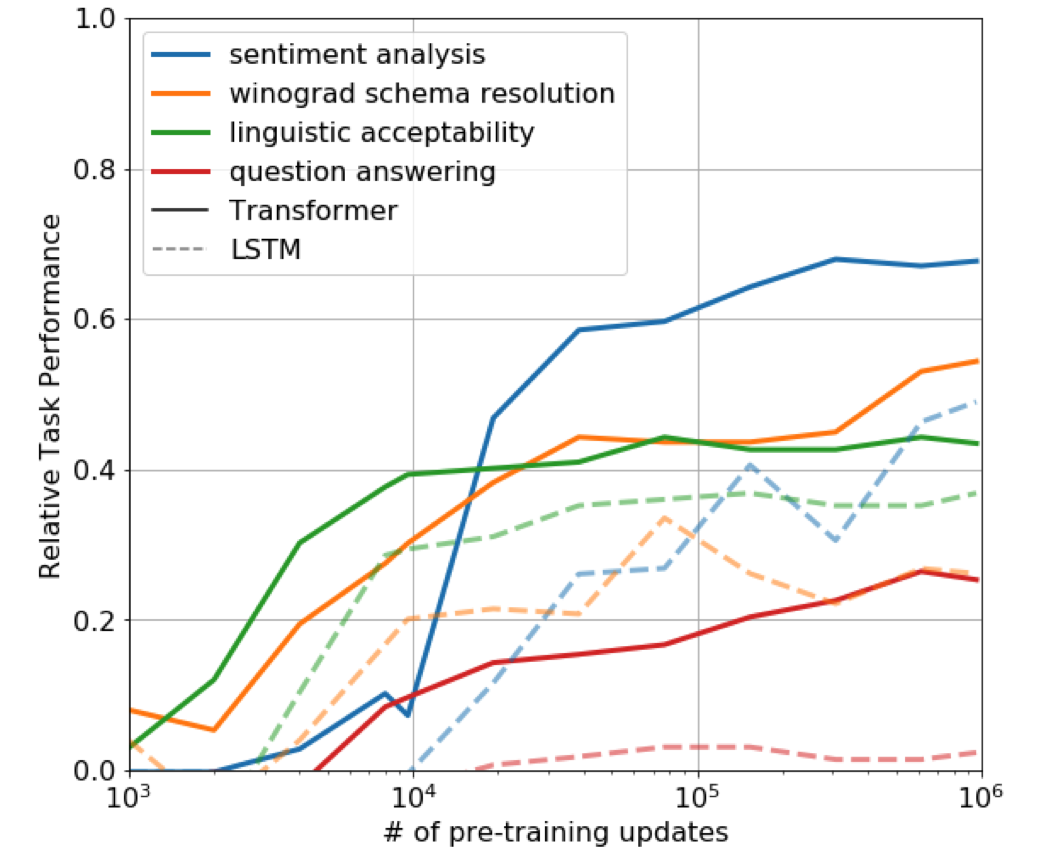
\includegraphics[width=\textwidth]{figures/gpt1-zs}
        \end{column}
        \begin{column}{0.6\textwidth}
            Heuristics for zero-shot prediction:
            \begin{itemize}
                \item Sentiment classification: [example] + very + \{positive, negative\} $\quad$ \blue{\em prompting}
                \item Linguistic acceptability: thresholding on log probabilities
                \item Multiple choice: predicting the answer with the highest log probabilities
            \end{itemize}
            \textbf{Learning dynamics}: zero-shot performance increases during pretraining
        \end{column}
    \end{columns}
\end{frame}

%lm as a general task solver
%- gpt2
%- gpt3
\begin{frame}
    {GPT-2: going beyond finetuning}
    Language Models are Unsupervised Multitask Learners \href{https://d4mucfpksywv.cloudfront.net/better-language-models/language-models.pdf}{[Radford et al., 2019]}
    
    \begin{itemize}
        \item \blue{Supervised learning}: models must be trained (finetuned) on a curated task dataset.
        \item They \red{fail to generalize} to out-of-distribution data (adversarial examples, robustness issues etc.) 
        \item A generalist model must be trained on {\em many} tasks---but how do we get the datasets?
        \item \textbf{Hypothesis}: a (large enough) LM should be able to infer and learn tasks demonstrated in natural language, effectively performing \blue{unsupervised multitask learning}
    \end{itemize}
\end{frame}

\begin{frame}
    {GPT-2 details}
    \begin{itemize}
        \item Similar to GPT-1 but {scaled up} (\blue{1.5B} parameters)
        \item Data (WebText): $\sim$40GB of \blue{web pages scraped from the internet} that was curated to include high-quality text
        \item Tokenization: BPE over byte sequences for \blue{universal text processing}. 
            \begin{itemize}
                \item Small base vocabulary (256)
                \item Can process any text data regardless of pre-processing, tokenization, or vocab size. 
            \end{itemize}
        \item \blue{Larger context} size (1024 tokens)
    \end{itemize}
\end{frame}

\begin{frame}
    {Zero-shot performance: cloze test}
    \begin{figure}
            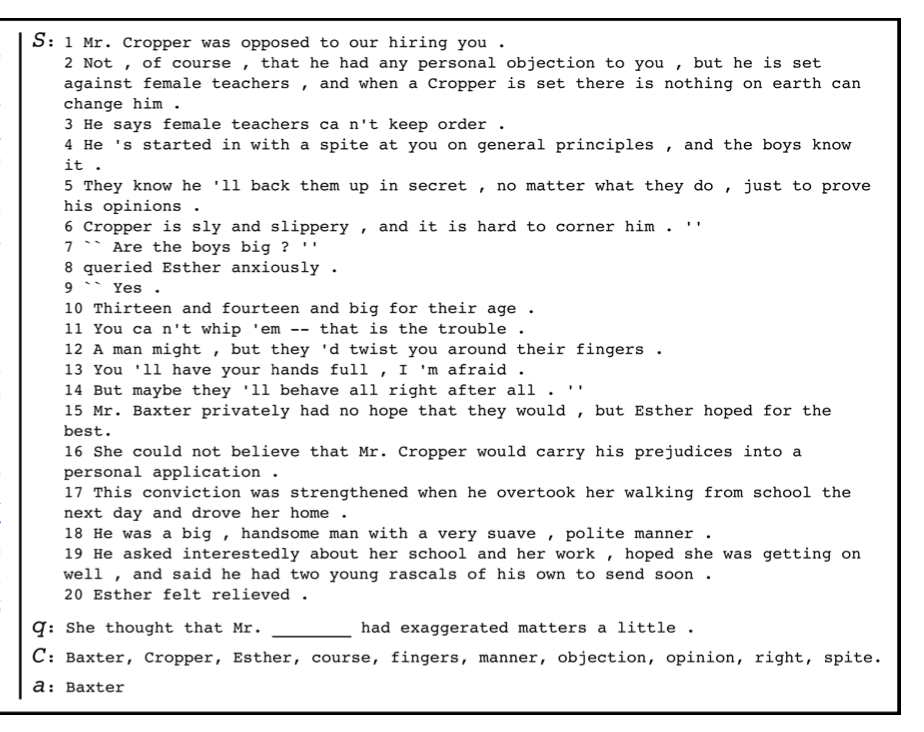
\includegraphics[width=0.45\textwidth]{figures/cbt}
            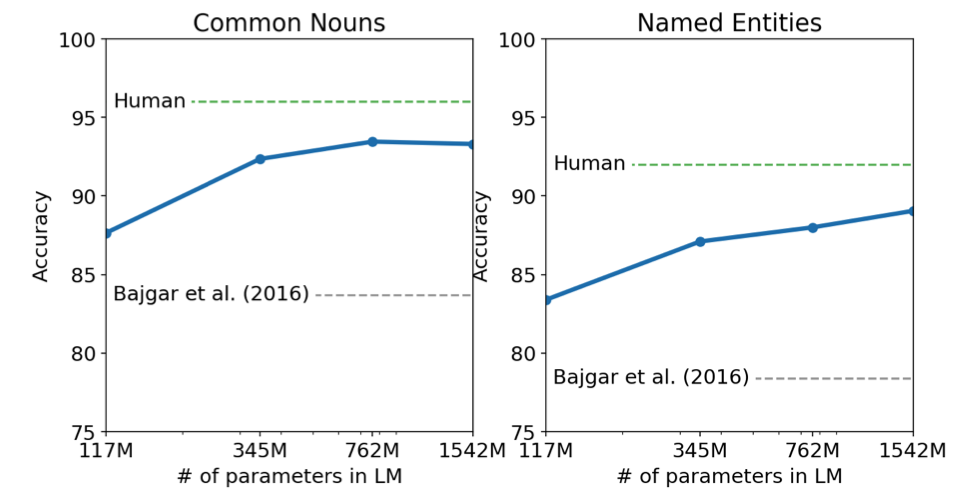
\includegraphics[width=0.52\textwidth]{figures/gpt2-cbt}
    \end{figure}
    Larger models quickly closes the gap with human performance
\end{frame}

\begin{frame}
    {Zero-shot performance: generative QA}
    \begin{figure}
        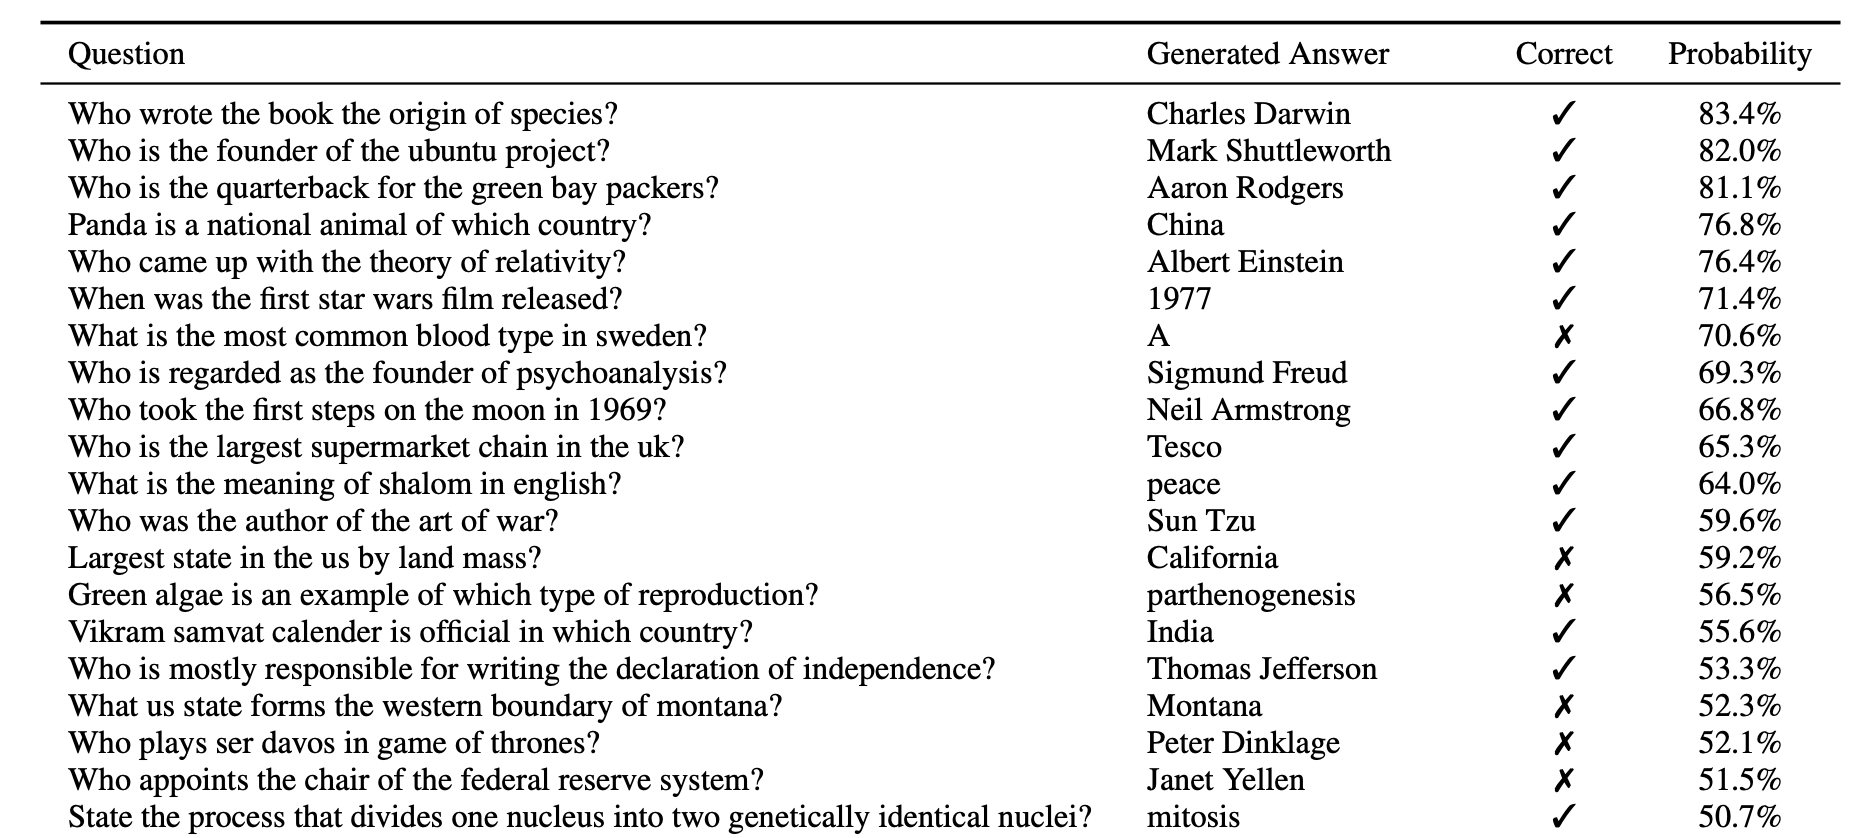
\includegraphics[width=\textwidth]{figures/gpt2-qa}
    \end{figure}
\end{frame}

\begin{frame}
    {Zero-shot performance: summarization}
    \begin{figure}
        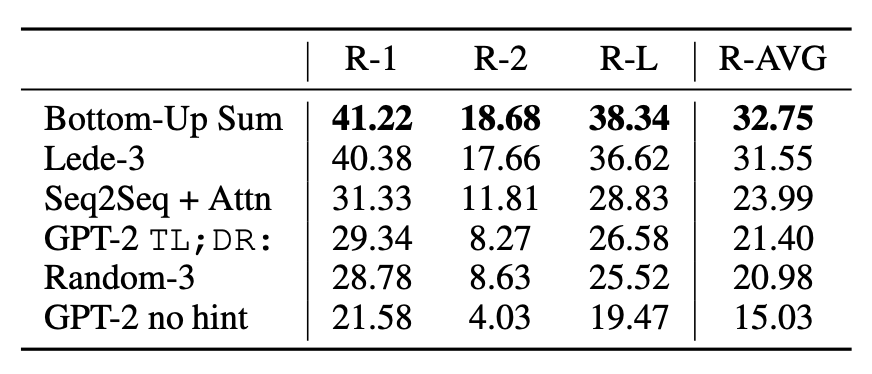
\includegraphics[width=0.5\textwidth]{figures/gpt2-sum}
    \end{figure}
    \begin{itemize}
        \item Challenge: not a ``native'' LM task
        \item Induce the task: [document] + \blue{[TL;DR]}
        \item Not much better than copying 3 random sentences from the document 
        \item Key question in the zero-shot paradigm: how do we tell the model what the intended task is?
    \end{itemize}
\end{frame}

\begin{frame}
    {Zero-shot performance: machine translation}
    
    \begin{itemize}
        \item Induce the task through a \blue{demonstration example}:
            $$
                \text{translation} \sim p(\cdot \mid \text{\blue{[french sentence] = [english sentence]}; [french sentence] =})
            $$
        \item WMT-14 French-English test set: 11.5 BLEU (worse than unsupervised MT)
        \item But, there's only 10MB french data in the 40GB training data!
            \begin{itemize}
                \item Typical unsupervised MT methods require crosslingual embeddings or monolingual corpora
            \end{itemize}
    \end{itemize}
\end{frame}

\begin{frame}
    {Has the model memorized everything?}
    Is there data contamination (test data in training set)?
    \begin{itemize}[<+->]
        \item Approach: check percentage of 8-grams that occur in both training and test data (using Bloom filters)
        \item Overlap is not higher than existing overlap on train and test in datasets
        \begin{itemize}
            \item Overlap between test and WebText: 3.2\%
            \item Overlap between test and their own training split: 5.9\%
        \end{itemize}
        \item Model performance does get better when the test data is in pretraining
        \begin{itemize}
            \item E.g., on CoQA, 3 F1 better on leaked documents 
        \end{itemize}
        \item In genreal, verifying and avoiding data contamination is an open research question
    \end{itemize}
\end{frame}

\begin{frame}
    {Has the model memorized everything?}
    Test the model on novel tasks:\\[-1em]
    \begin{figure}
        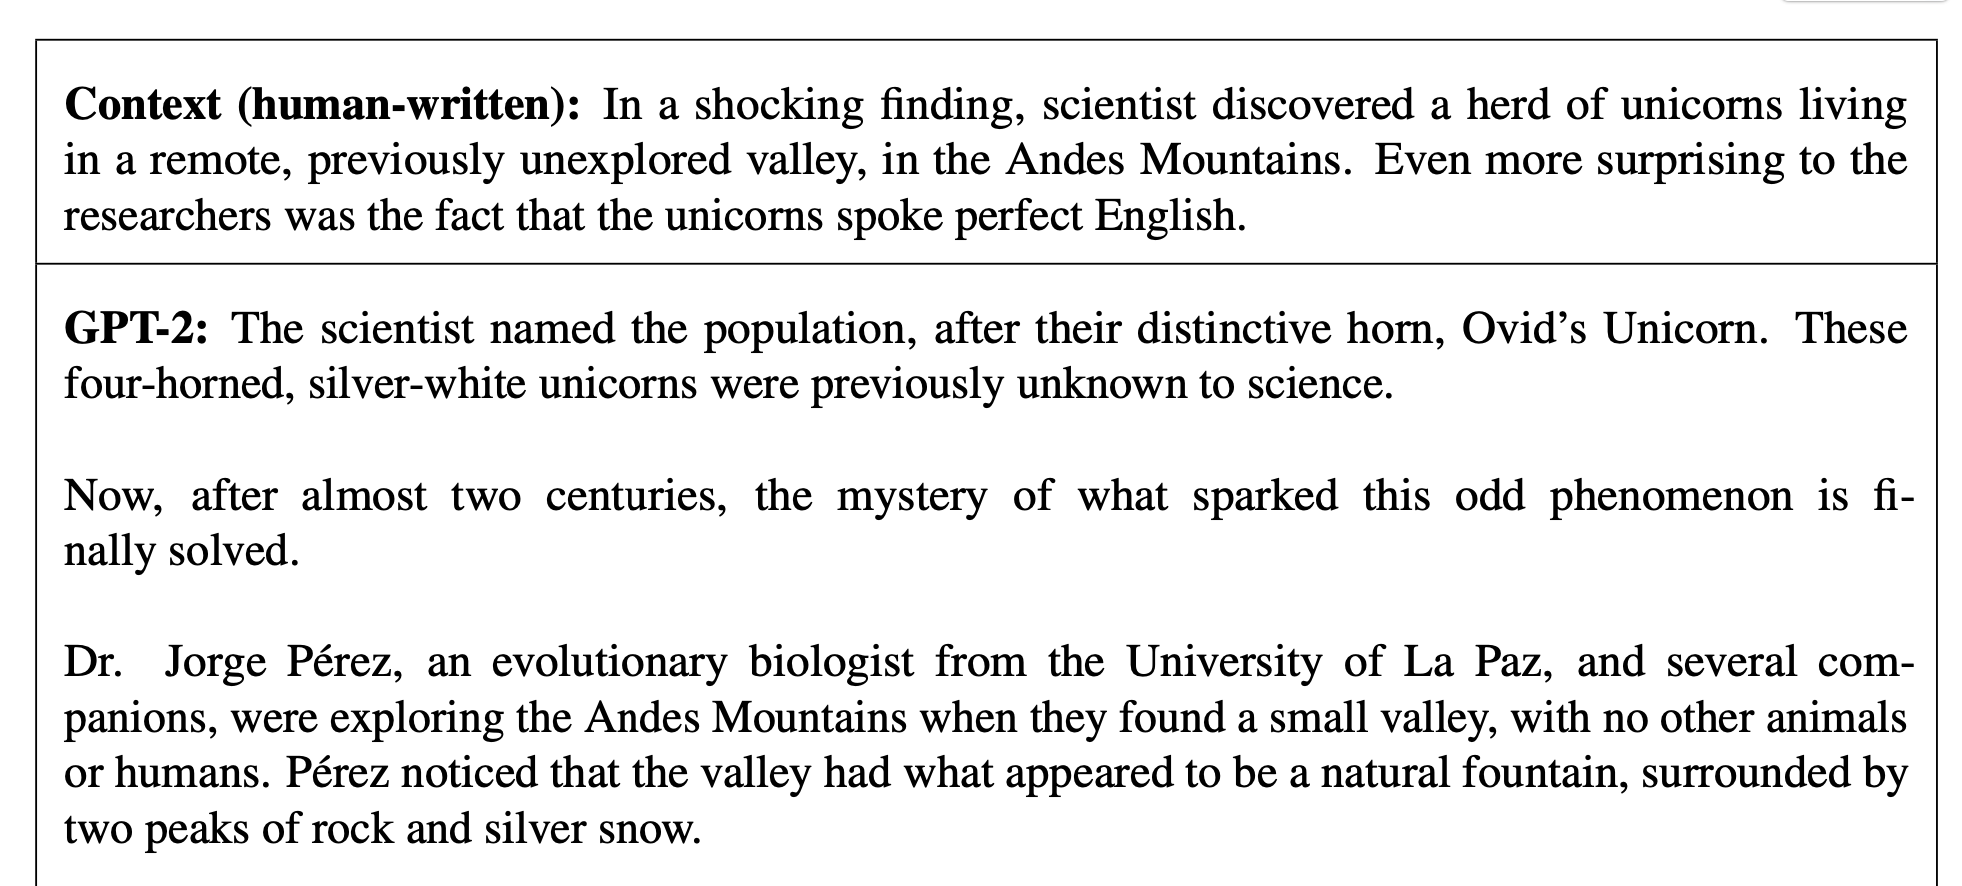
\includegraphics[width=\textwidth]{figures/gpt2-gen}
    \end{figure}
\end{frame}

\begin{frame}
    {GPT-3: scaling up}
    \begin{itemize}
        \item GPT-2 shows promise for zero-shot learning, but performance is still unsatisfying
        \item GPT-3 \blue{scales up} model size, data size and diversity, and number of training steps
        \item Notable improvement in zero-shot and few-shot performance
        \item Inducing a task through natural language \blue{task descriptions} 
    \end{itemize}
    \begin{figure}
        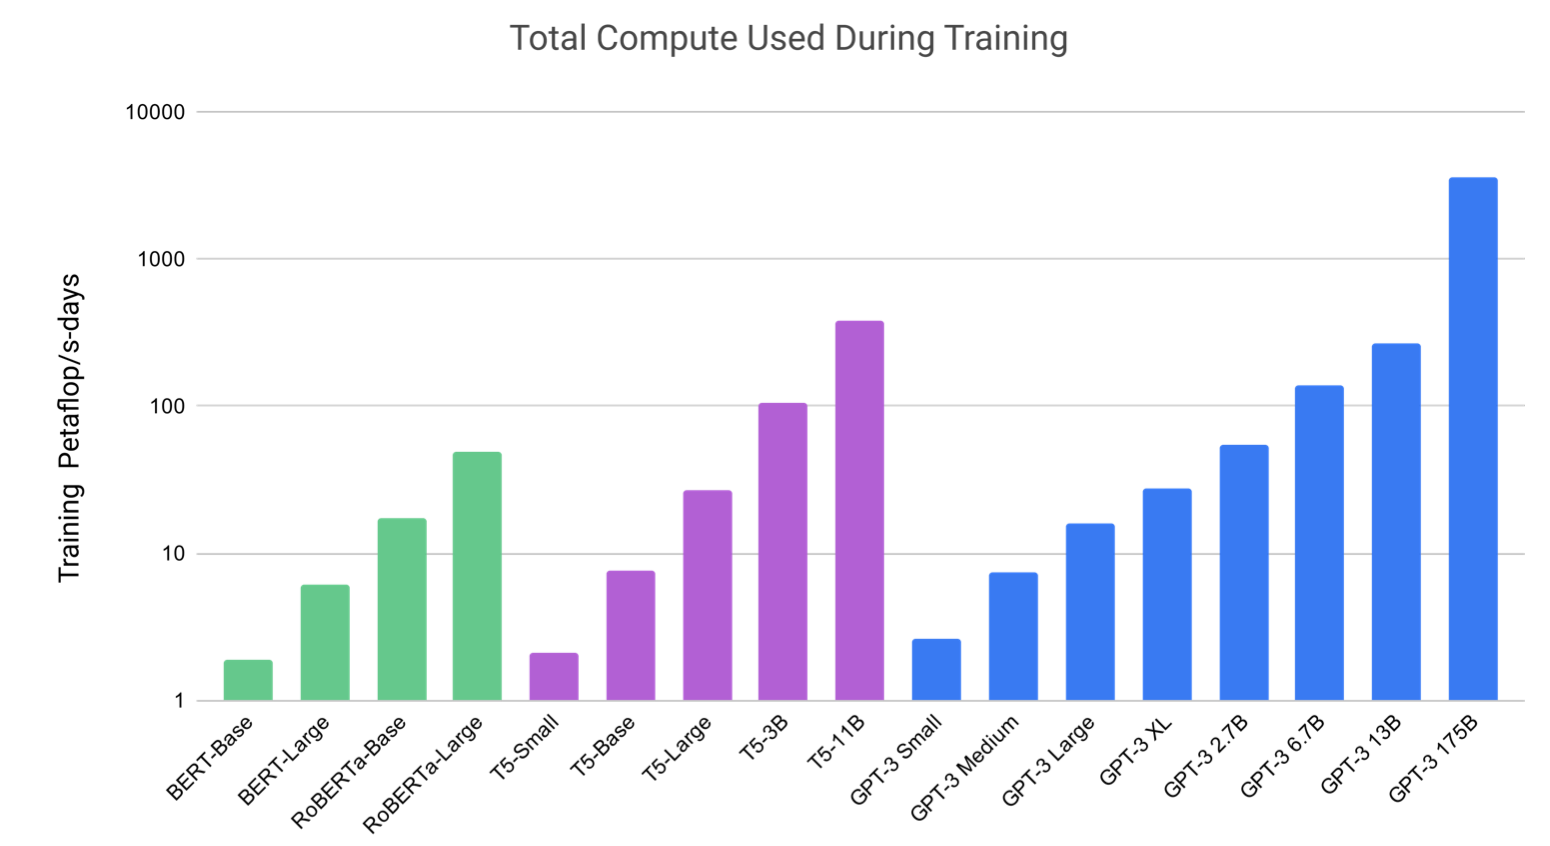
\includegraphics[height=0.6\textheight]{figures/gpt3-compute}
    \end{figure}
\end{frame}

\begin{frame}
    {Training data}
    \begin{figure}
        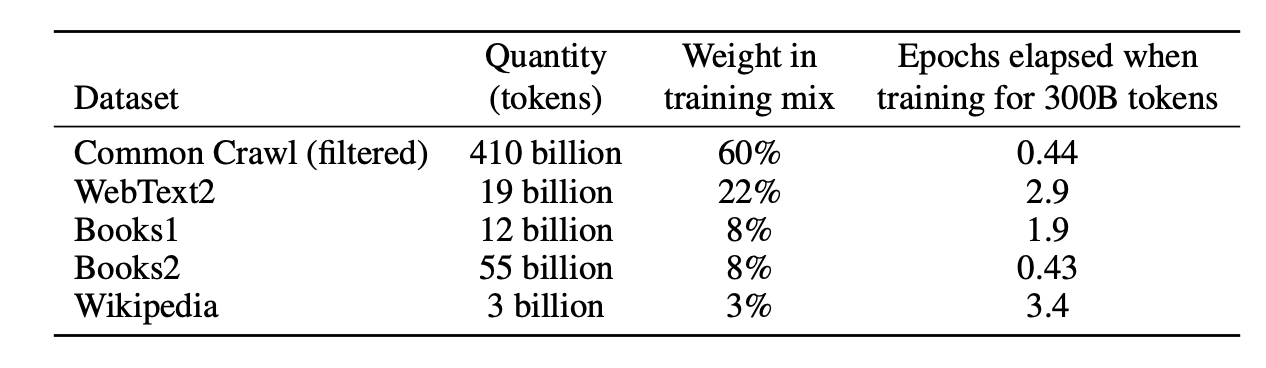
\includegraphics[height=0.4\textheight]{figures/gpt3-data}
    \end{figure}
Key challenge: data quality control
    \begin{itemize}
        \item \blue{Filter} CommonCrawl based on similarity to high-quality reference corpora 
        \item Fuzzy \blue{deduplication}: avoid redundancy and data contamination
        \item Mix in known \blue{high quality data}
        \item Upsampling high quality data during training
    \end{itemize}
\end{frame}

\begin{frame}
    {Evaluation settings}
    \begin{figure}
        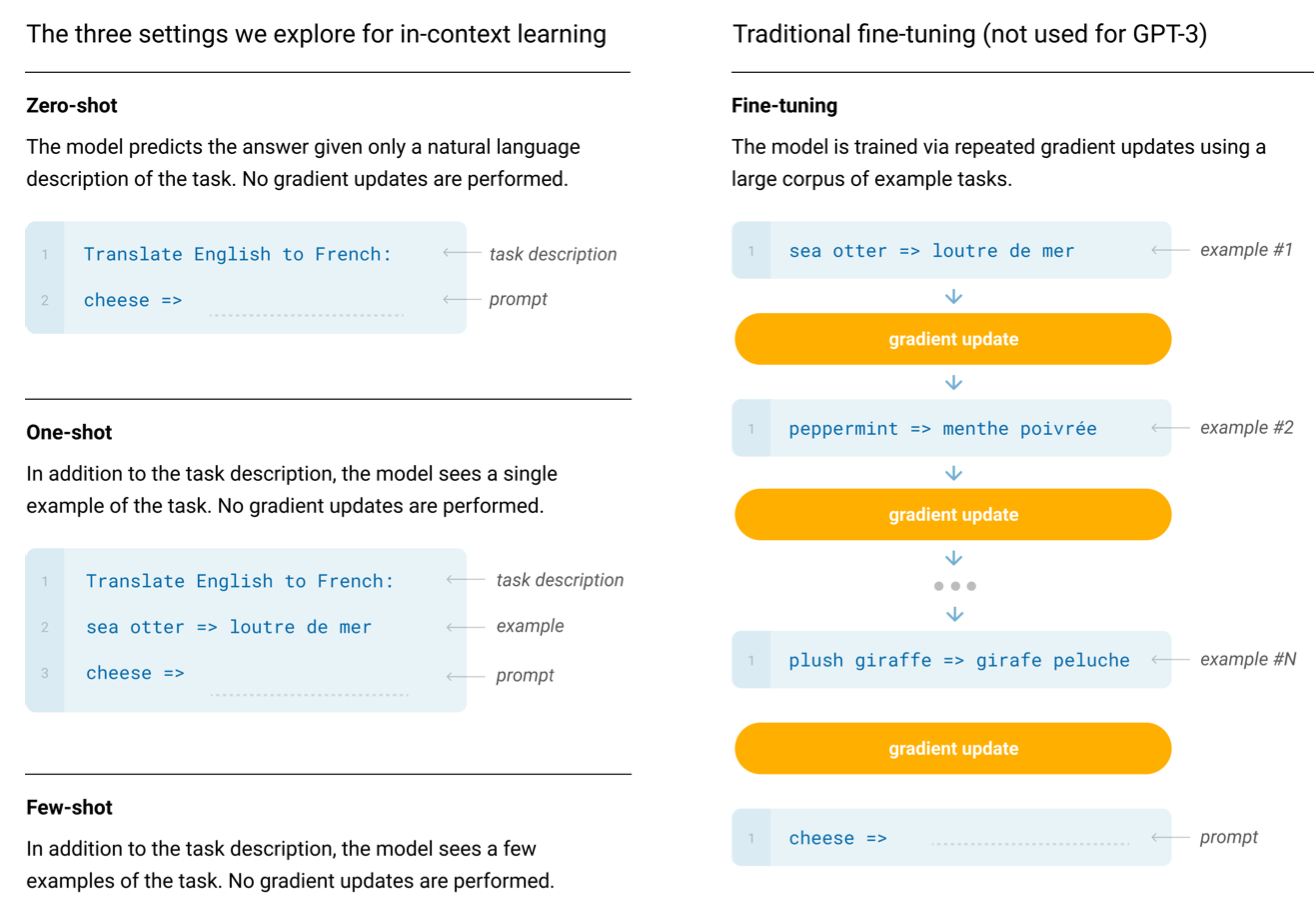
\includegraphics[height=0.9\textheight]{figures/gpt3-inf}
    \end{figure}
\end{frame}

\begin{frame}
    {Results: natural language understanding}
    \begin{figure}
        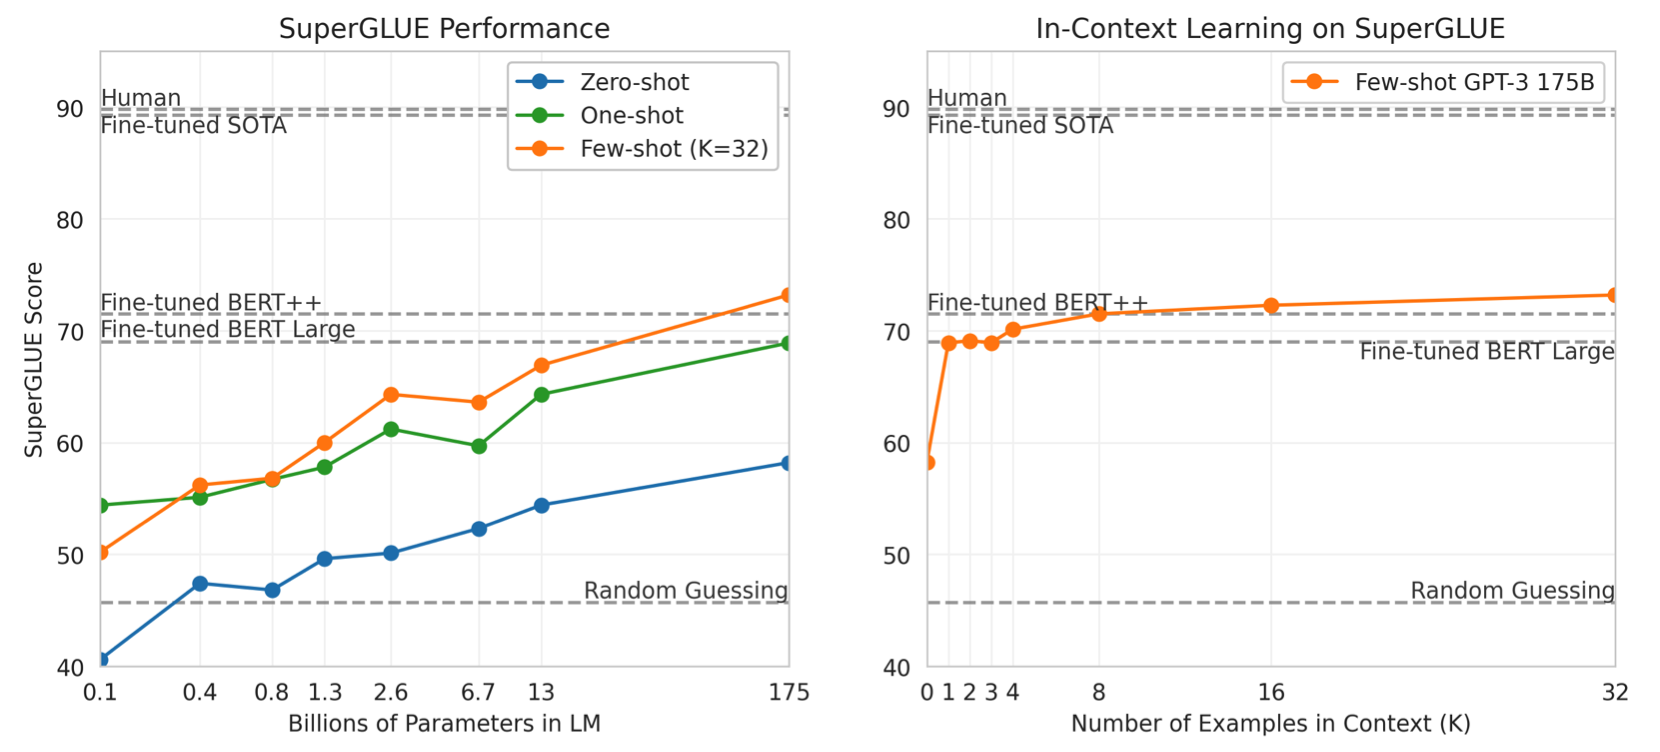
\includegraphics[width=\textwidth]{figures/gpt3-superglue}
    \end{figure}
    Comparable to supervised results
\end{frame}

\begin{frame}
    {Results: few-shot machine translation}
    \begin{figure}
        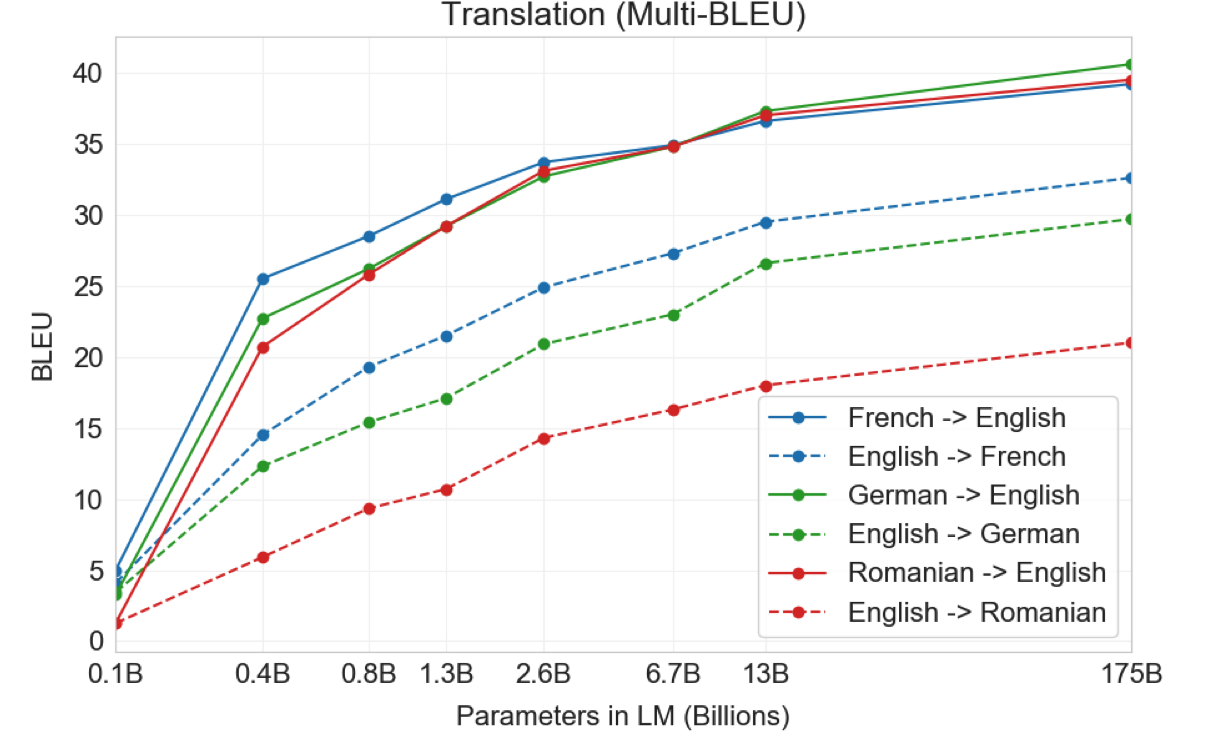
\includegraphics[height=0.6\textheight]{figures/gpt3-translation}
    \end{figure}
    \begin{itemize}
        \item Pretraining data: 93\% English, 7\% other languages
        \item Zero-shot is still worse than unsupervised MT
        \item But even giving one examples significantly boosts the result (+7 BLEU points)
        \item Results much better when translation into English
    \end{itemize}
\end{frame}

\begin{frame}
    {Results: arithmetic}
    \begin{figure}
        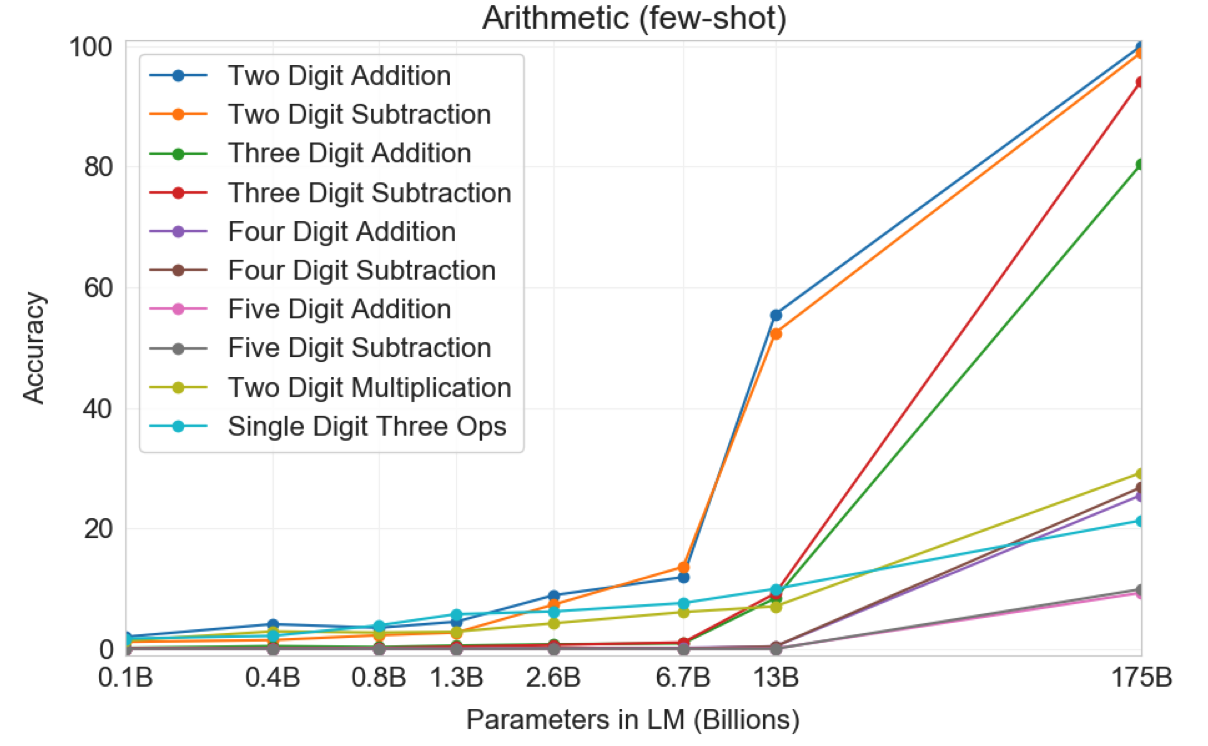
\includegraphics[height=0.6\textheight]{figures/gpt3-arith}
    \end{figure}
    \begin{itemize}
        \item "Emergent" ability at certain model scale
        \item Not systemic: works better on frequent numbers \href{https://arxiv.org/abs/2202.07206}{[Razeghi et al., 2022]}
    \end{itemize}
\end{frame}

\begin{frame}
    {Results: generation}
    \begin{figure}
        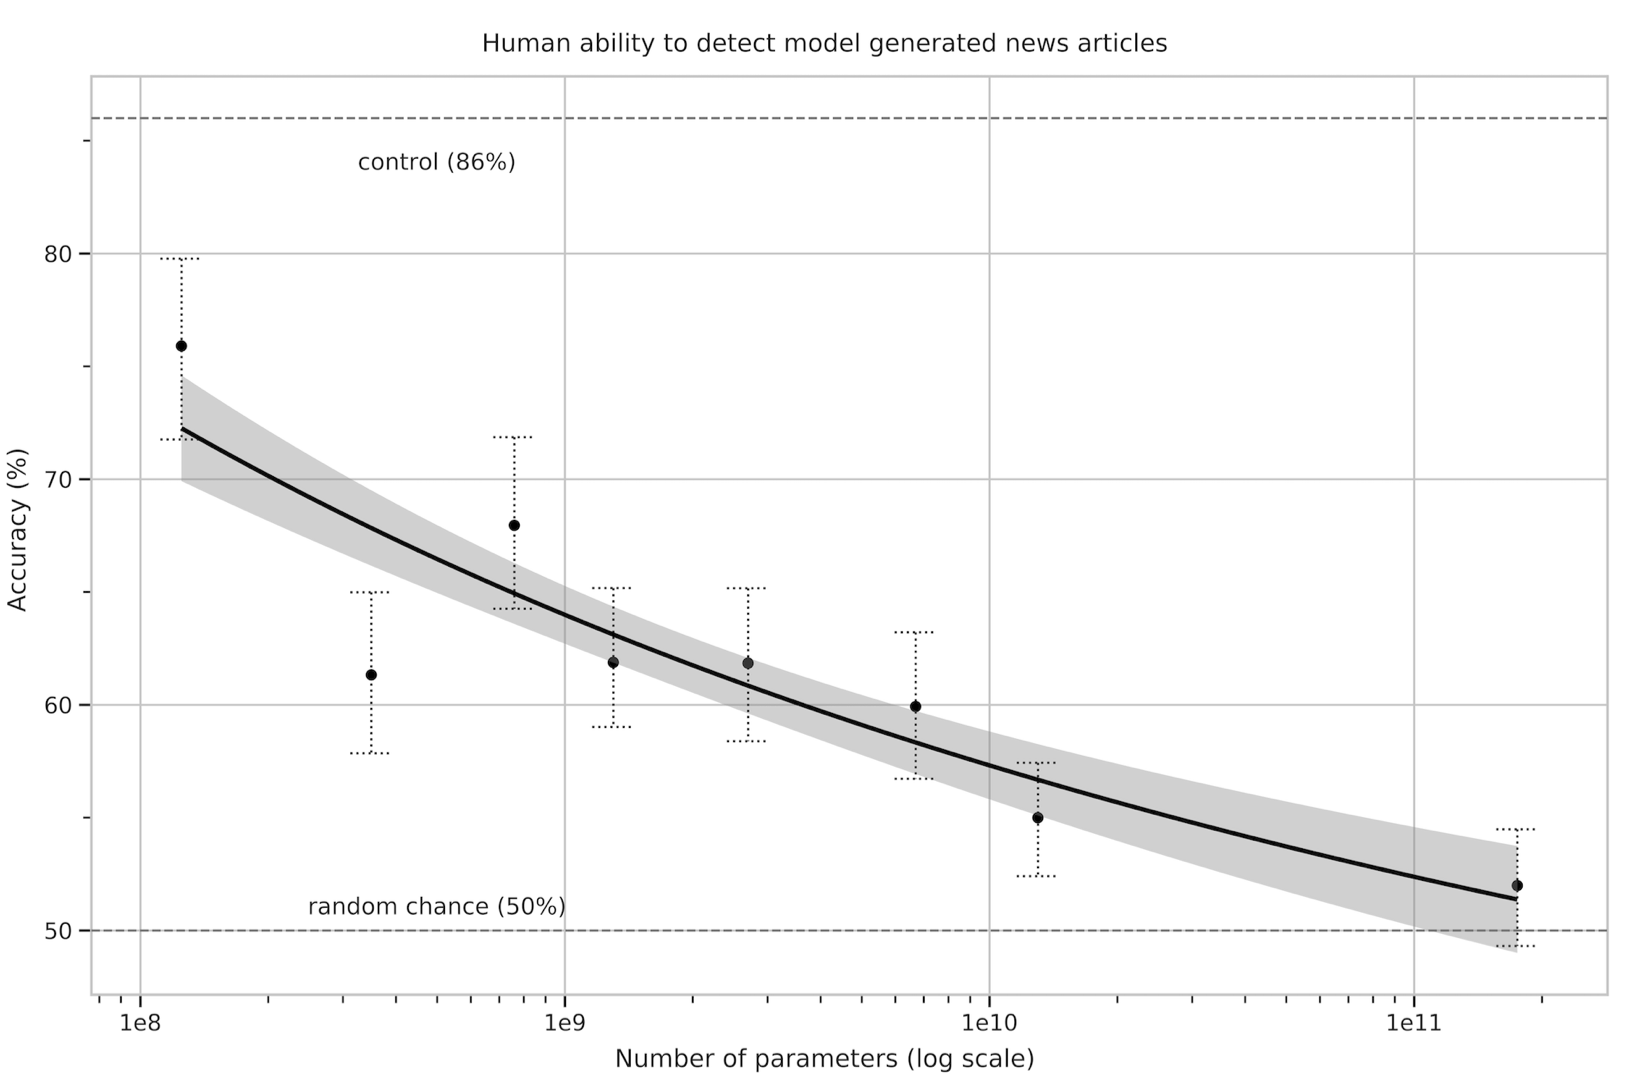
\includegraphics[height=0.6\textheight]{figures/gpt3-gen}
    \end{figure}
    Generated text is hard to detect from human-written text
\end{frame}

\begin{frame}
    {Analysis: data contamination}
    \begin{figure}
        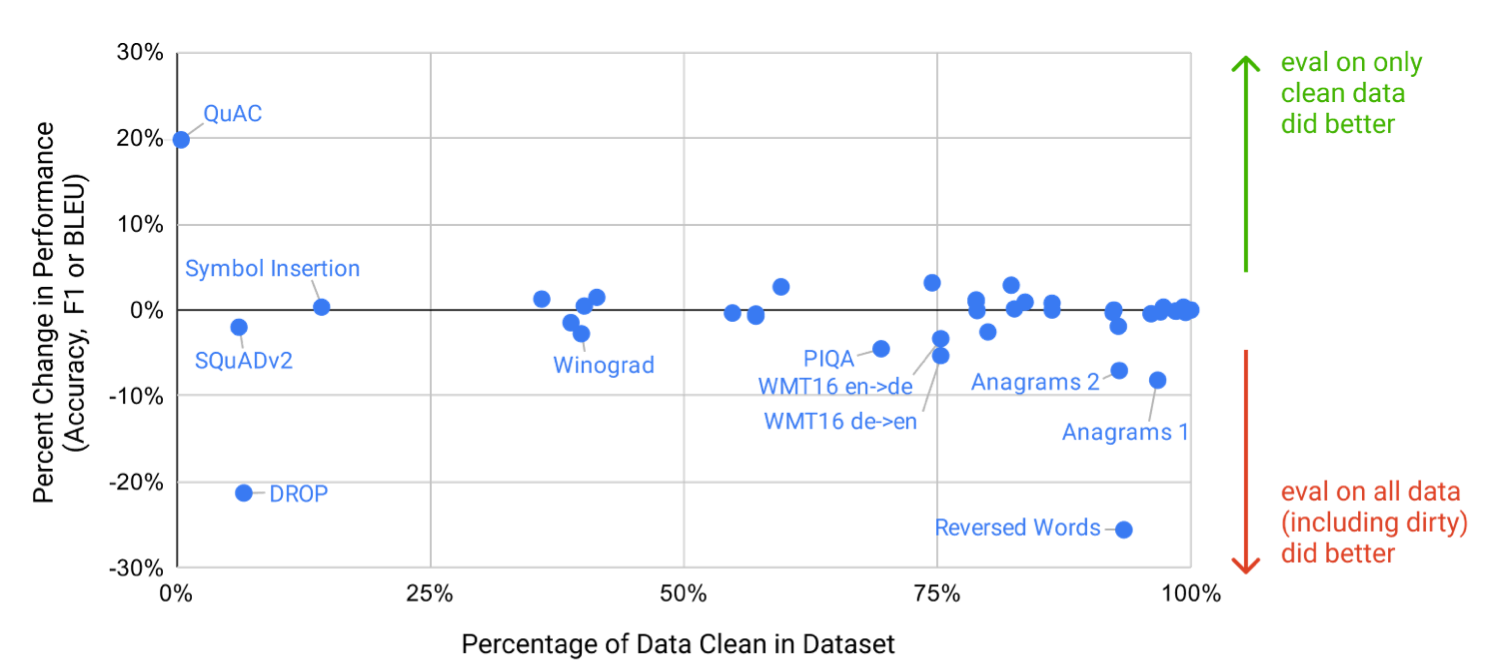
\includegraphics[height=0.6\textheight]{figures/gpt3-contamination}
    \end{figure}
    \begin{itemize}
        \item Overlap can be large (e.g., many reading comprehension articles come from wikipedia) 
        \item Result on clean part of the benchmark doesn't change much
    \end{itemize}
\end{frame}

\begin{frame}
    {Conclusion}
    \begin{itemize}
        \item A perfect language model on all human-written text can do all text-based tasks
        \item New behaviors that are not written in the training objective emerge (e.g., in-context learning)
        \item Open questions:
            \begin{itemize}
                \item How much are they memorizing vs generalizing?
                \item How do new abilities emerge?
                \item How to mitigate harmful, toxic, biased responses?
            \end{itemize}
    \end{itemize}
\end{frame}

\end{document}
